% Created 2026-04-23 Thu 12:09
% Intended LaTeX compiler: lualatex
\DocumentMetadata{lang = en-US,pdfversion = 2.0,pdfstandard = ua-2,tagging = on,tagging-setup = {math/setup=mathml-SE},}
\documentclass[11pt]{article}
\usepackage{amsmath}
\usepackage{fontspec}
\usepackage{graphicx}
\usepackage{longtable}
\usepackage{wrapfig}
\usepackage{rotating}
\usepackage[normalem]{ulem}
\usepackage{capt-of}
\usepackage{hyperref}
\usepackage[margin=1in]{geometry}
\usepackage{fontspec}
\usepackage{verbatim, multicol, tabularx,}
\usepackage{amsmath, amsthm, amssymb, stmaryrd, latexsym, bm, listings, qtree}
\usepackage{framed}
\usepackage{xcolor,colortbl}
\usepackage{media9}
\usepackage[export]{adjustbox}
\usepackage{algorithm}
\usepackage[noend]{algpseudocode}
\usepackage{tikz,pgfplots}
\usetikzlibrary{shapes.geometric}
\let\oldquote=\quote
\let\endoldquote=\endquote
\colorlet{shadecolor}{cyan!15}
\renewenvironment{quote}{\begin{shaded*}\begin{oldquote}}{\end{oldquote}\end{shaded*}}
% From https://tex.stackexchange.com/questions/7032/good-way-to-make-textcircled-numbers
\newcommand*\circled[1]{\tikz[baseline=(char.base)]{\node[shape=circle,draw,inner sep=2pt] (char) {#1};}}
\DeclareMathOperator*{\argmin}{arg\!min}
\DeclareMathOperator*{\argmax}{arg\!max}
\lstset{frame=tb, aboveskip=1mm, belowskip=0mm, showstringspaces=false, columns=flexible, basicstyle={\scriptsize\ttfamily}, numbers=left, frame=single, breaklines=true, breakatwhitespace=true}
\hypersetup{colorlinks=true,urlcolor=blue}
\usepackage{tagpdf}
\tagpdfsetup{activate-all}
\tagpdfsetup{math/alt/use}
\usepackage{polyglossia}
\setdefaultlanguage[variant=en-US]{english}
\author{Christopher Simpkins}
\date{Kennesaw State University}
\title{Artificial Intelligence\\\medskip
\large Nondeterministic Search}
\hypersetup{
 pdfauthor={Christopher Simpkins},
 pdftitle={Artificial Intelligence},
 pdfkeywords={},
 pdfsubject={Artificial Intelligence Nondeterministic Search},
 pdfcreator={Emacs 30.2 (Org mode 9.7.11)}, 
 pdflang={English}}
\begin{document}

\maketitle
\section{Nondeterministic Search (AIMA 4.3-4.5)}
\label{sec:org5e9df36}

So far we've learned about search in fully observable, deterministic, known environments.  In this lesson we consider:

\begin{itemize}
\item environments with nondeterministic actions,
\item partially observable environments, and
\item unknown environments.
\end{itemize}
\section{Nondeterministic Actions: The Erratic Vacuum World}
\label{sec:org22cd9a4}




In the erratic vacuum world, the Suck action works as follows:

\begin{itemize}
\item When applied to a dirty square the action cleans the square and sometimes cleans up dirt in an adjacent square, too.
\item When applied to a clean square the action sometimes deposits dirt on the carpet.
\end{itemize}

So the result of each action is a set, e.g.:

\begin{equation*}
\text{Results}(1,Suck) = \{5, 7\}
\end{equation*}

That set of states that the agent believes is possible, \{5, 7\}, is called a \textbf{belief state}.





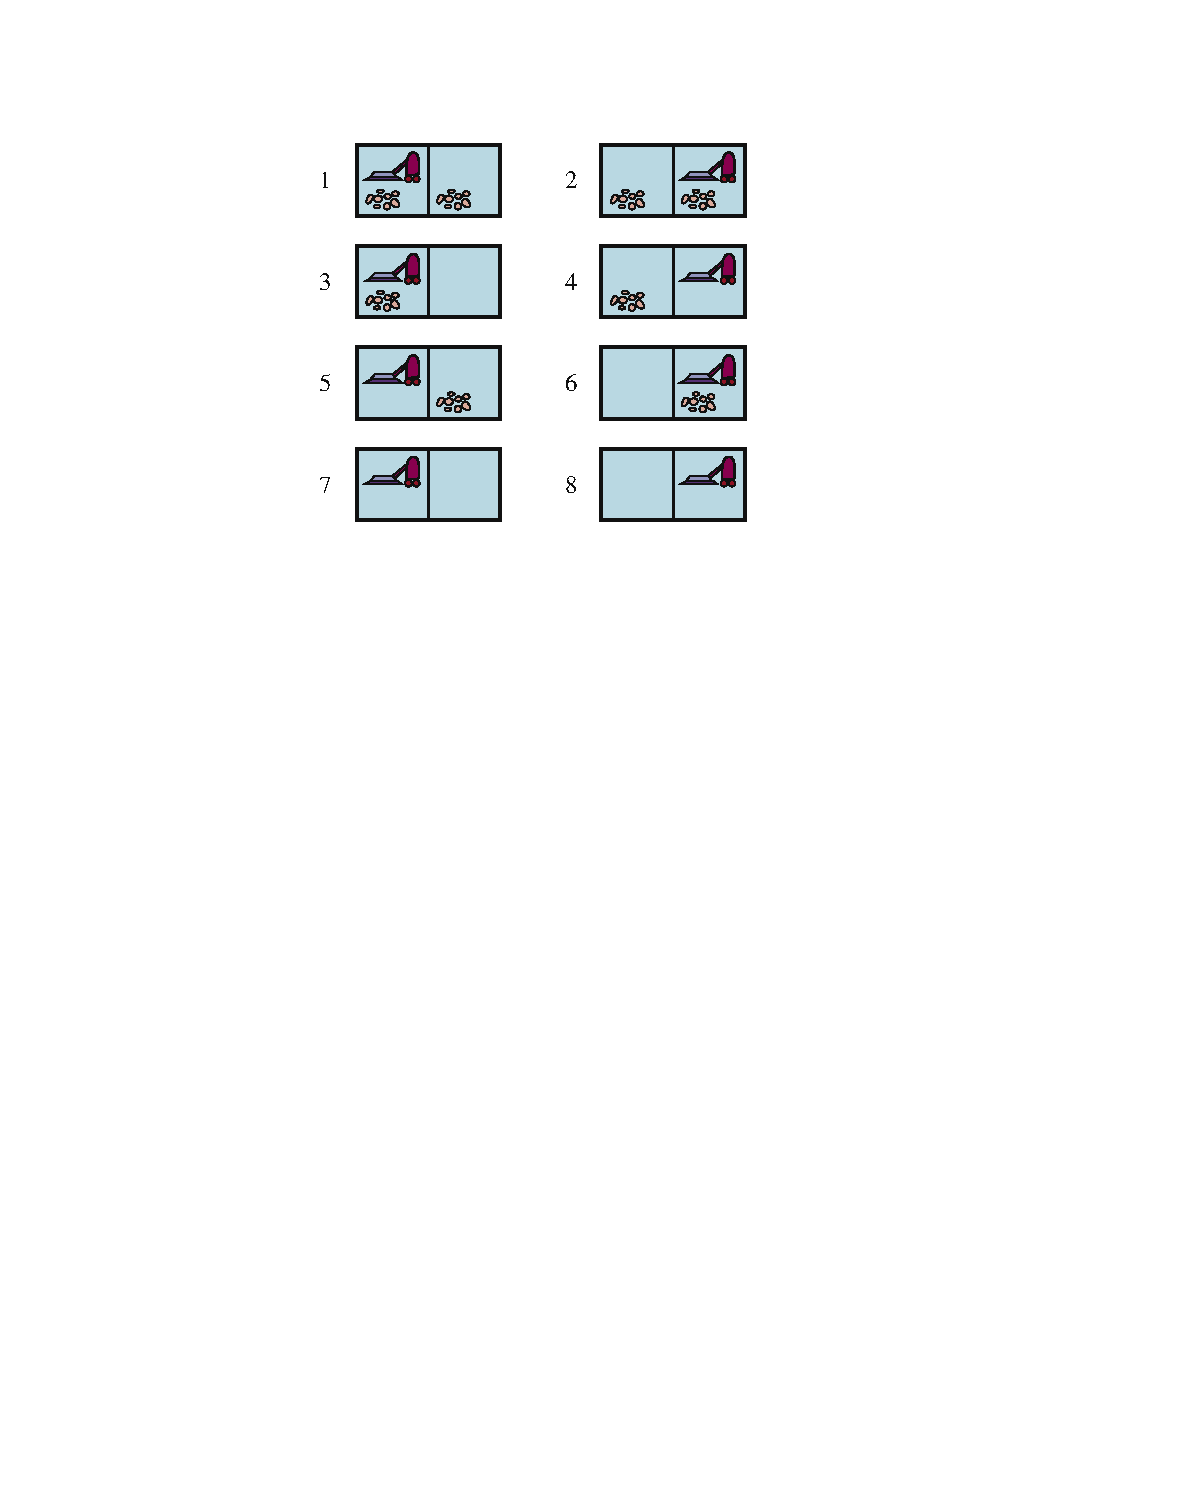
\includegraphics[alt={aima fig 04_09 vacuum states},width=0.75\linewidth]{aima-fig-04_09-vacuum-states.pdf}
\section{A Factored Representation}
\label{sec:org74dcd17}

Let's depart from the book for a few slides and, instead of using an index into a vector of states, create a factored representation for clarity.

\begin{itemize}
\item `left-condition` \(\in\) \{\texttt{CLEAN}, \texttt{DIRTY}\}
\item `right-condition` \(\in\) \{\texttt{CLEAN}, \texttt{DIRTY}\}
\item `vacuum-location` \(\in\) \{\texttt{LEFT}, \texttt{RIGHT}\}
\item State representation: ``
\end{itemize}

So


`Results(1,Suck) = \{5, 7\}`

becomes

`Results(, Suck) = \{, \}`


Note that the factored representation is easier for us to read (don't have to look up states in a table), but the search algorithms we're considering here treat these states as atomic.
\section{Conditional Plans}
\label{sec:org7631eef}

A conditional plan, a.k.a. \textbf{contingency plan}, is a plan that specifies action selection based on the observed state while executing the plan.

\begin{itemize}
\item In a fully-observable, deterministic world contingencies are not necessary -- a plan is just a sequence of actions.
\item We need conditional/contingency plans in environments that are partially observable or nondeterministic.
\end{itemize}

Consider the start state, ``.  Due to the environment's nondeterminism, not possible to find a sequence of actions guaranteed to solve the problem.  But this simple conditional plan does:


`[Suck, if State ==  then [Right, Suck] else []]`
\section{AND-OR Search Trees}
\label{sec:orgc63dbfc}




\begin{itemize}
\item Branch on agent's action: \textbf{OR nodes}, shown as states.
\item Branch on environment's outcome: \textbf{AND nodes}, shown as circles with arc linking branches to possible outcome states (when > 1).
\item A plan includes actions for OR nodes, and conditional actions for AND nodes that contain more than one state.
\end{itemize}

Trace this conditional plan through the tree on the right.

`[Suck,`
`if State ==  then [Right, Suck]`
`else []]`





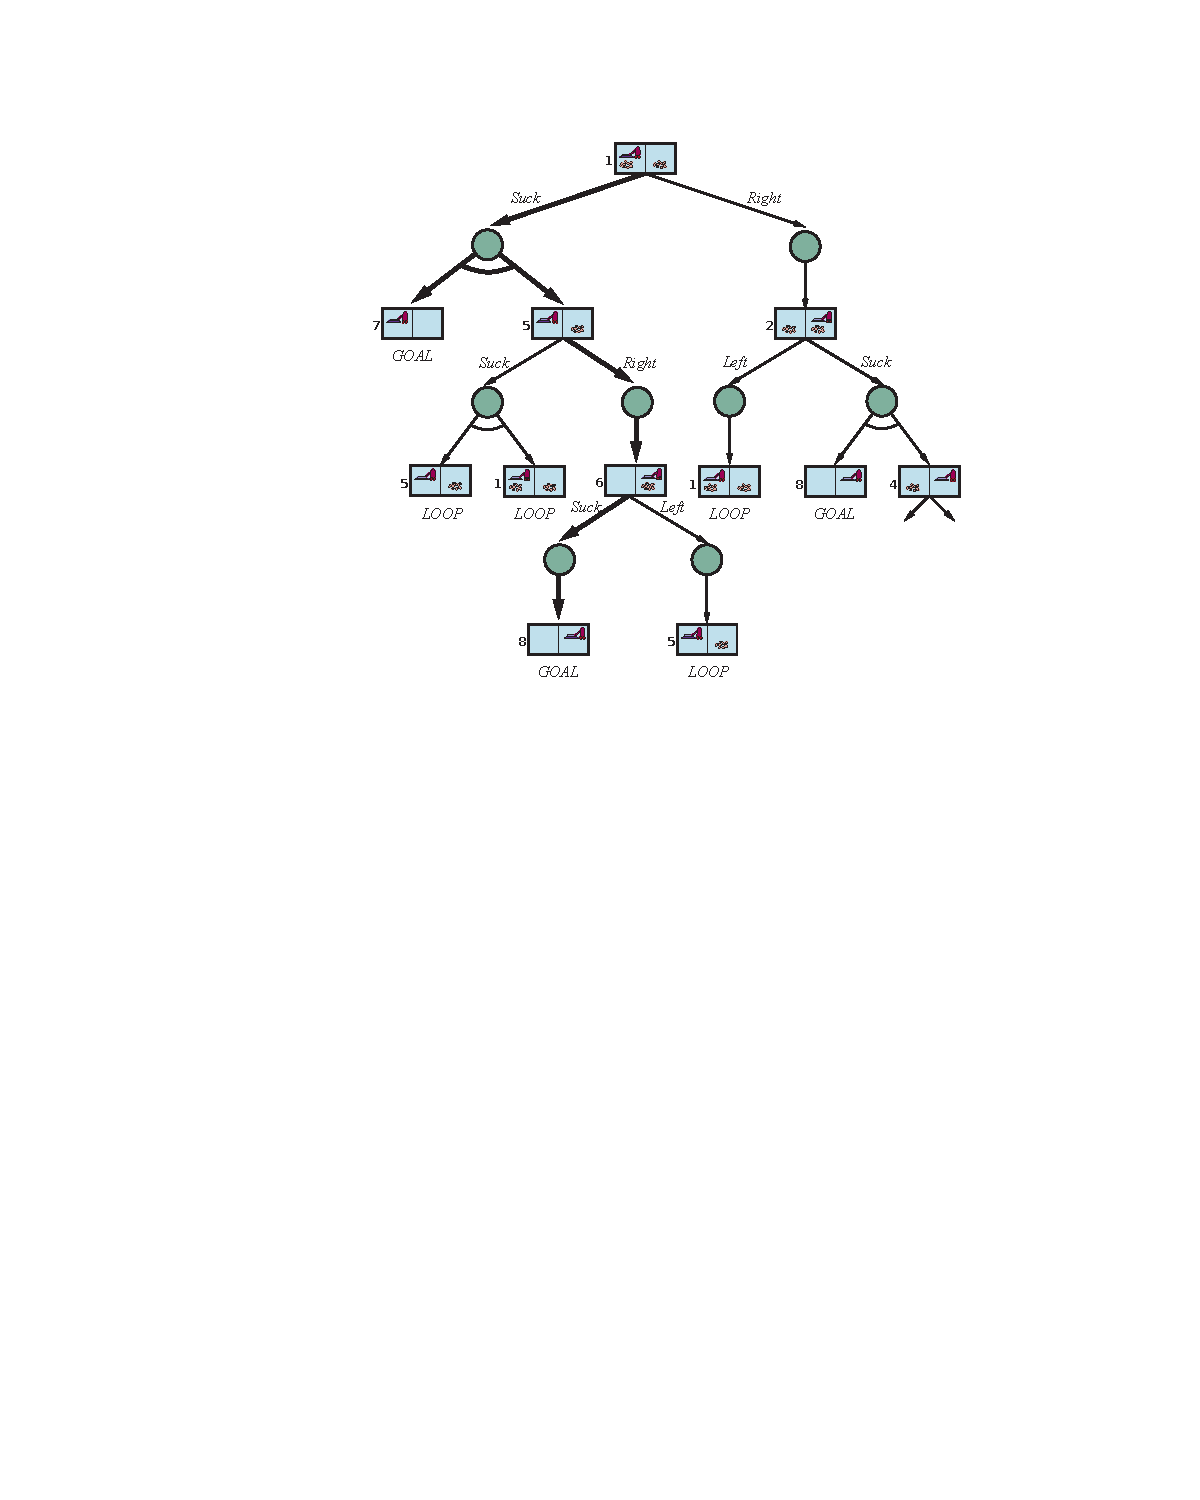
\includegraphics[alt={aima fig 04_10 vacuum and or search tree},height=3.6in]{aima-fig-04_10-vacuum-and-or-search-tree.pdf}
\section{Slippery Vacuum World}
\label{sec:org40c6433}




\begin{itemize}
\item Like deterministic vacuum world, but a movement action may result in no movement.
\end{itemize}


`Results(, Right) =`
`    \{, \}`


\begin{itemize}
\item Do deal with nondetermnistic movements we need cyclic plans.  Use a \textbf{while} construct:
\end{itemize}


`[Suck,`
` while State ==  do Right,`
` Suck]`






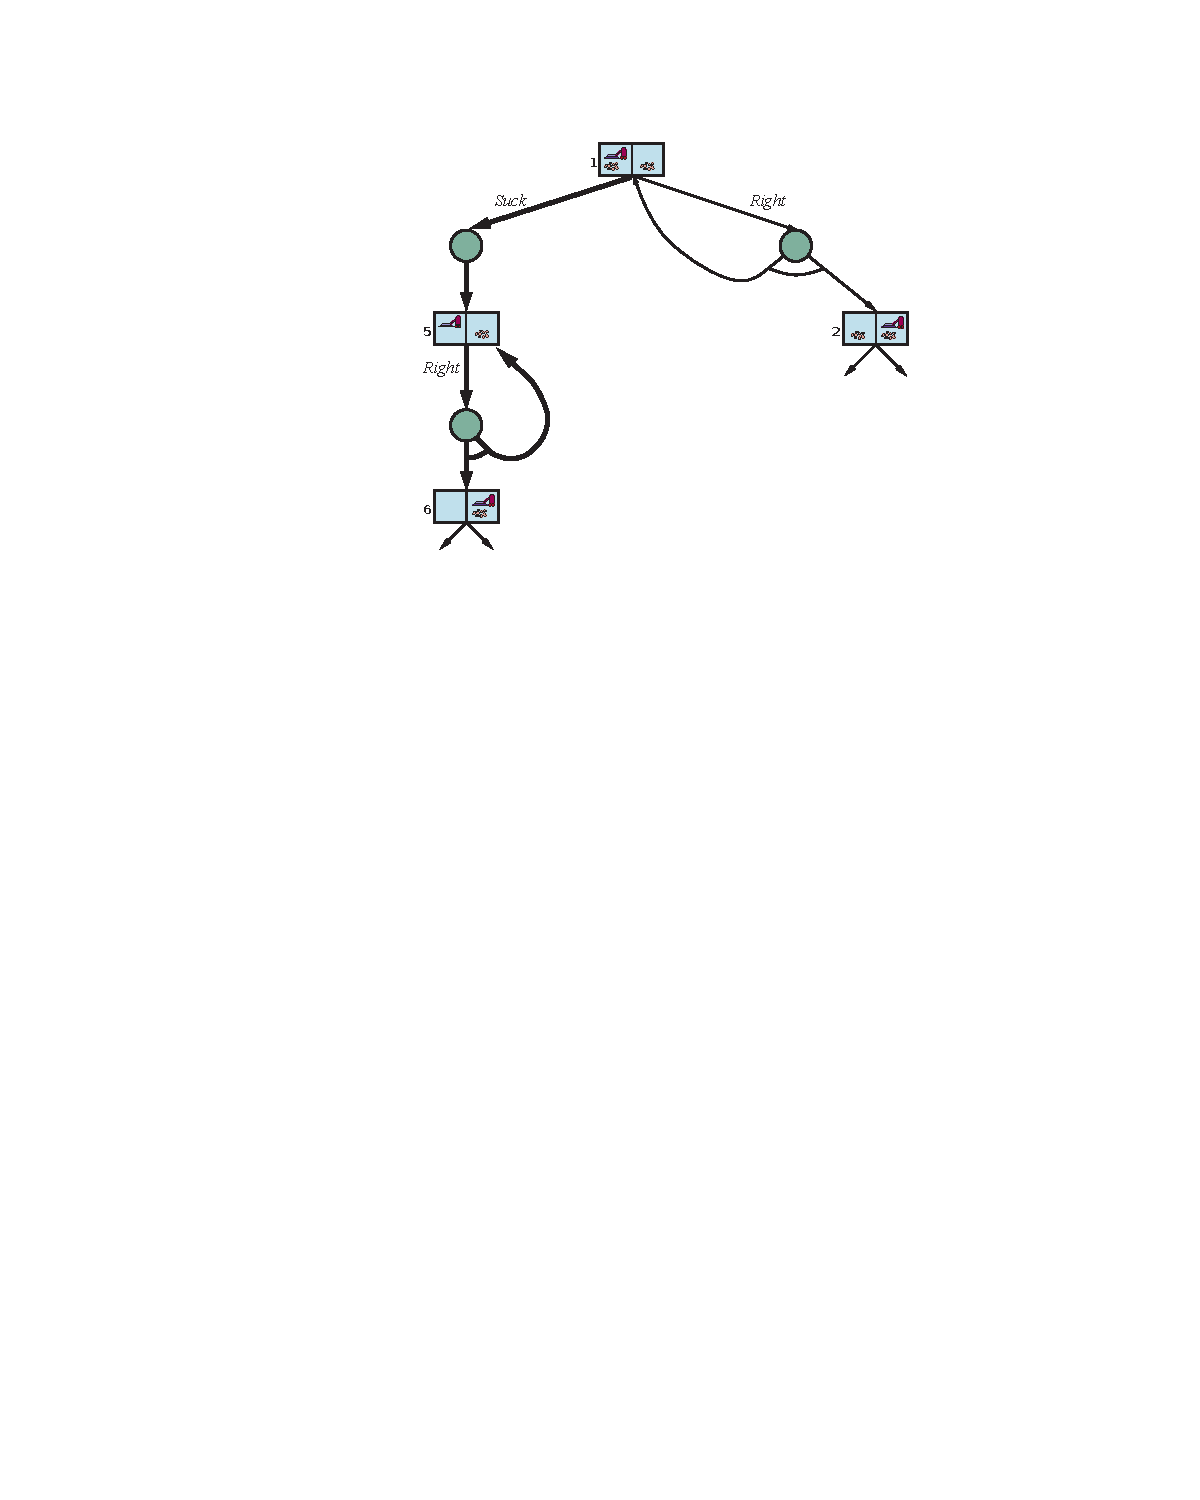
\includegraphics[alt={aima fig 04_12 slippery vacuum search graph},height=3.6in]{aima-fig-04_12-slippery-vacuum-search-graph.pdf}
\section{Search in Sensorless Environments}
\label{sec:orgc6c9e1f}





Now let's turn to uncertainty in the state observations, first with a sensorless world.

Sensorless, a.k.a. conformant, problems are surprisingly common.

\begin{itemize}
\item Manufacturing: orienting parts regardless of initial position.
\item Medicine: applying broadly applicable treatments without running tests.
\end{itemize}

Consider a sensorless version of the (deterministic) vacuum world. Assume that the agent knows the geography of its world, but not its own location or the distribution of dirt.

Given an initial belief state is \{1,2,3,4,5,6,7,8\}.

\begin{itemize}
\item After [Right], belief state is \{2,4,6,8\}
\item After [Right,Suck] belief state is \{4,8\}.
\item After [Right,Suck,Left,Suck], belief state is \{7\}.
\end{itemize}

We say that the agent can \textbf{coerce} the world into state 7.





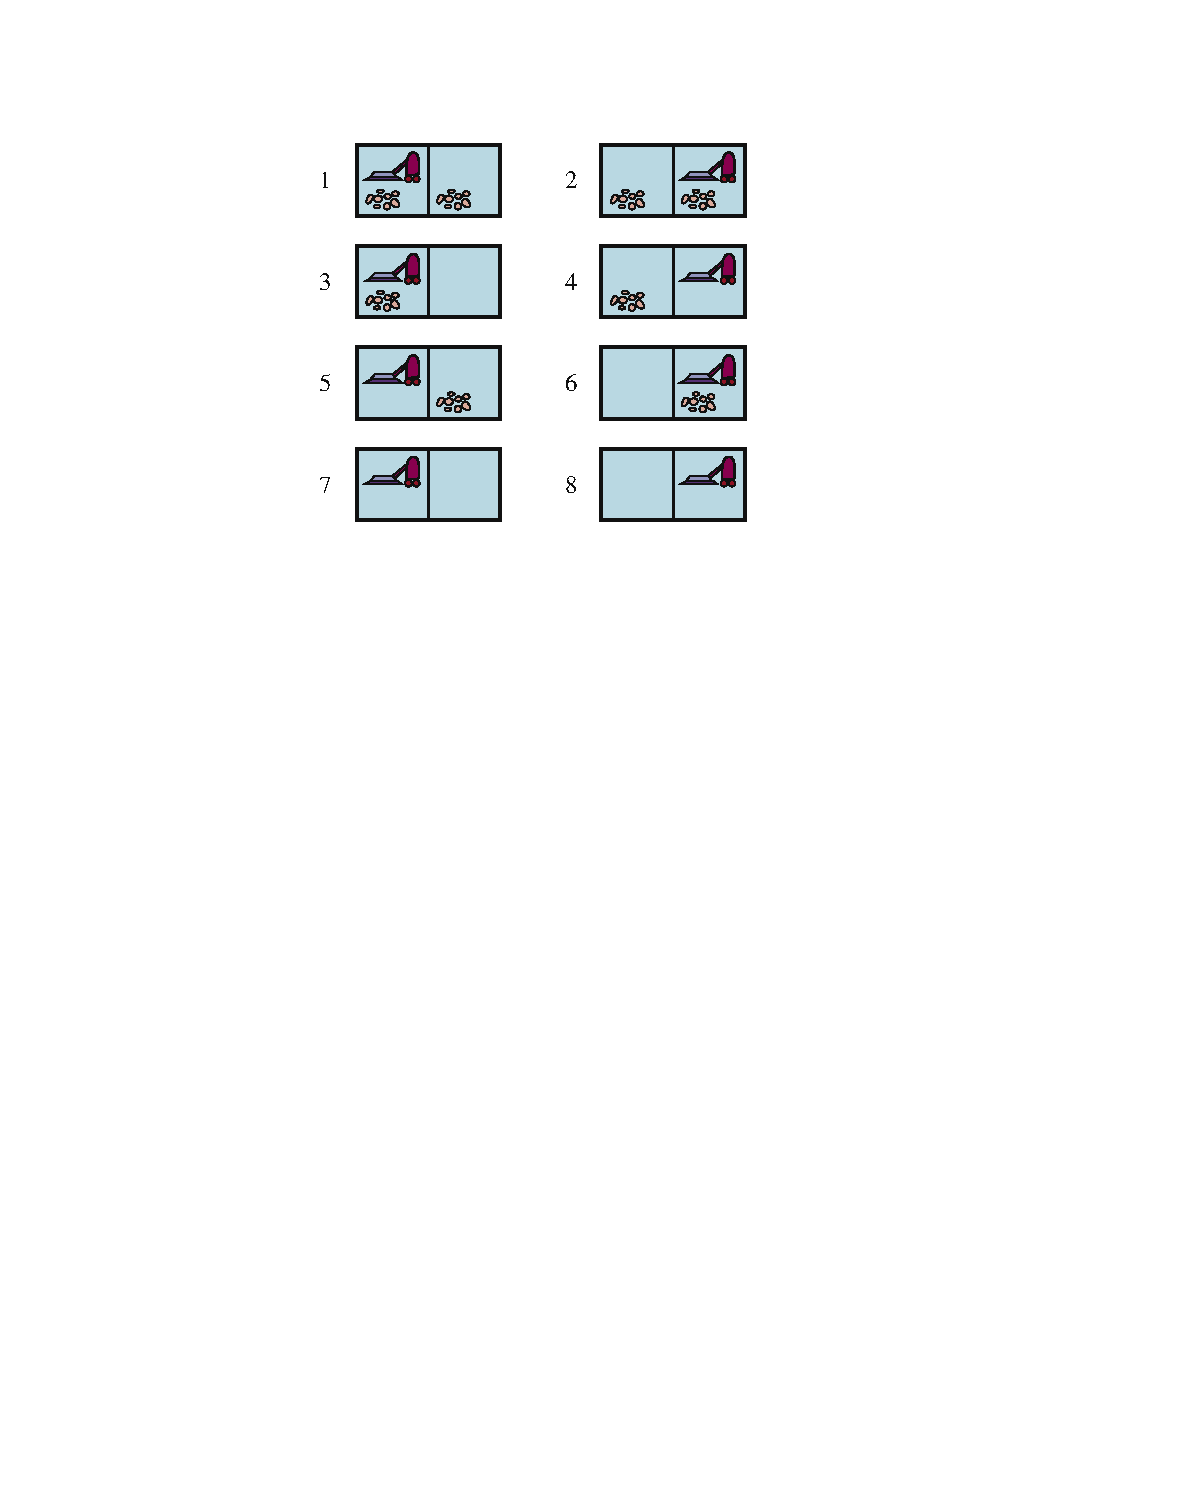
\includegraphics[alt={aima fig 04_09 vacuum states},width=0.75\linewidth]{aima-fig-04_09-vacuum-states.pdf}
\section{Search Algorithms for Sensorless Environments}
\label{sec:org2bf481f}

Instead of creating new algorithms, we transform the original problem into a belief state problem.

The original problem, \(P\), has components \(Actions_P\), \(Result_P\) etc., and the belief-state problem has the following components:

\begin{itemize}
\item \textbf{States}: The belief-state space contains every possible subset of the physical states. If \(P\) has \(N\) states, then the belief-state problem has \(2^N\) belief states, although many of those may be unreachable from the initial state (see next slide).

\item \textbf{Initial state}: Typically the belief state consisting of all states in \(P\), although in some cases the agent will have more knowledge than this.

\item \textbf{Actions}: \(Actions(b) = \bigcup_{s \in b} Actions_P(s)\) or \(Actions(b) = \bigcap_{s \in b} Actions_P(s)\)

\item \textbf{Transition model}: For deterministic actions, the new belief state has one result state
\end{itemize}
for each of the current possible states.  With nondeterminism, the new belief state consists of all the possible results of applying the action to any of the states in the current belief state.

\begin{itemize}
\item \textbf{Goal test}.  We aim to \textbf{necessarily} achieve the goal.

\begin{itemize}
\item The agent \textbf{possibly} achieves the goal if \(\exists s \in b : IsGoal_P(s)\).
\item The agent \textbf{necessarily} achieves the goal if \(\forall s \in b : IsGoal_P(s)\).
\end{itemize}

\item \textbf{Action cost}: If the same action can have different costs in different states, then the cost of taking an action in a given belief state could be one of several values. For now we assume that the cost of an action is the same in all states and so can be transferred directly from the underlying physical problem.
\end{itemize}
\section{Reachable States in Sensorless Vacuum World}
\label{sec:orgf7c8727}

Only 12 reachable belief states out of \(2^8 = 256\) possible belief states.





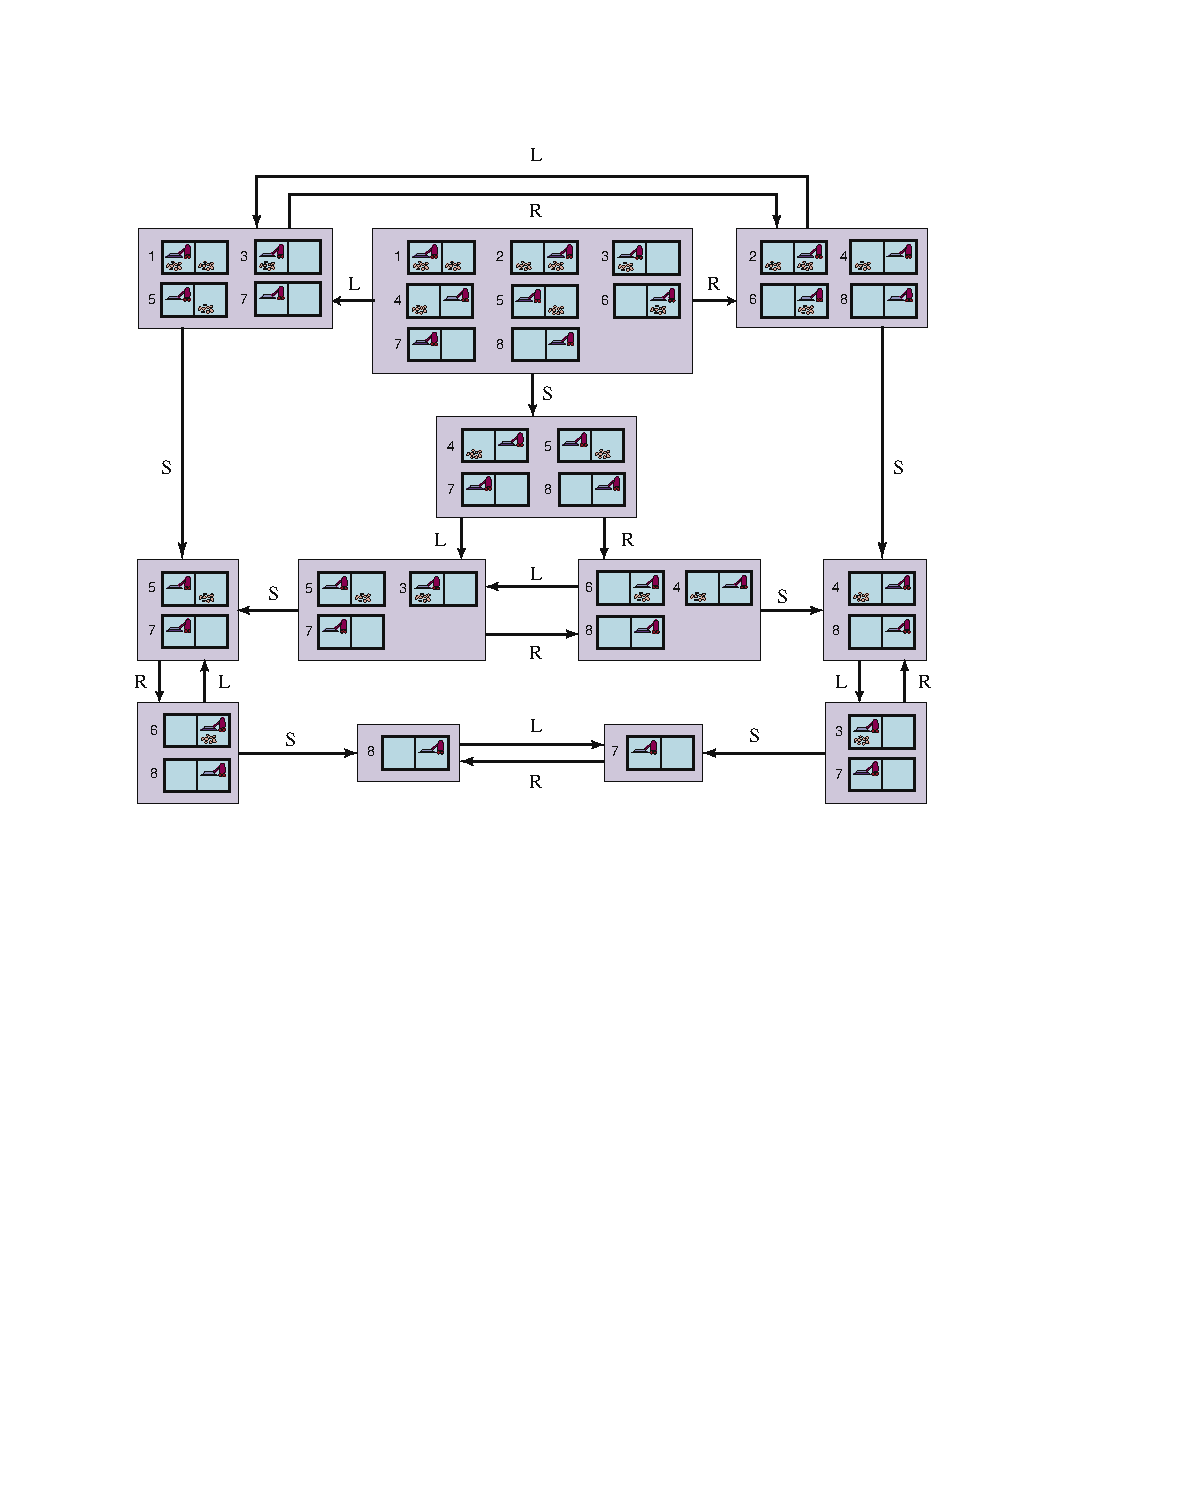
\includegraphics[alt={aima fig 04_14 reachable sensorless vacuum belief states},height=3.2in]{aima-fig-04_14-reachable-sensorless-vacuum-belief-states.pdf}





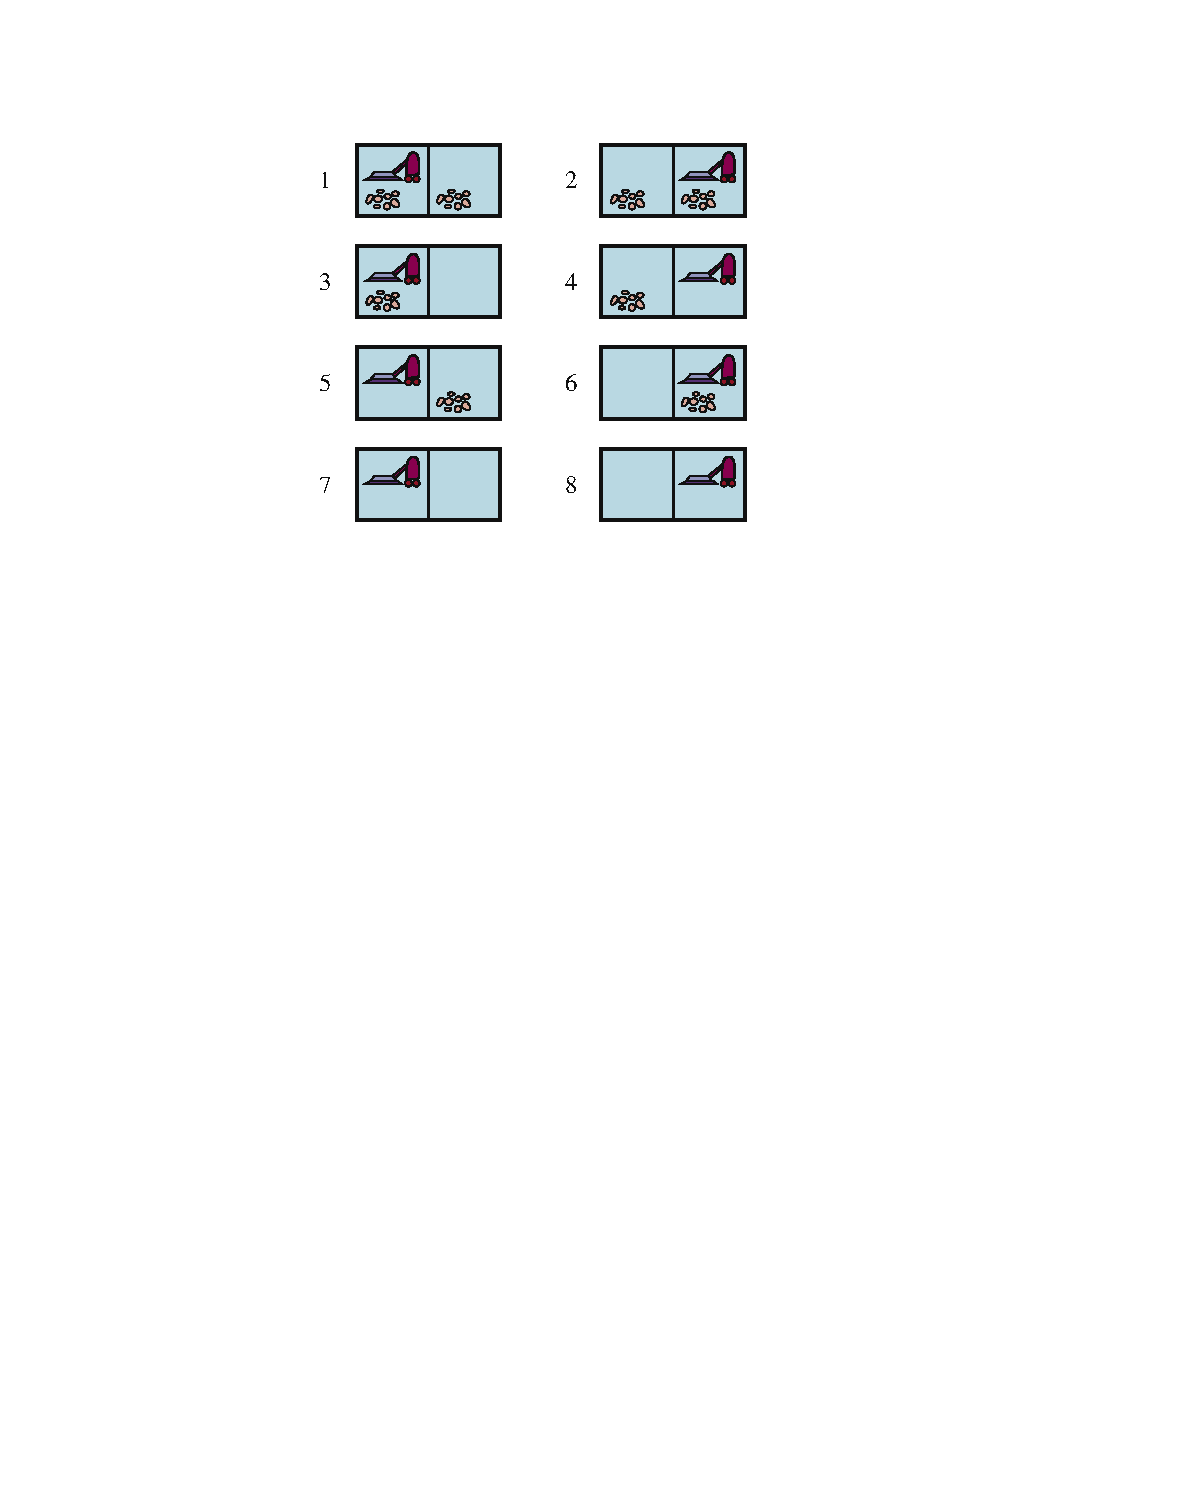
\includegraphics[alt={aima fig 04_09 vacuum states},width=0.75\linewidth]{aima-fig-04_09-vacuum-states.pdf}
\section{Actions in Sensorless Environments}
\label{sec:org53d6792}

\begin{itemize}
\item \textbf{Actions}: If \(b = \{s_1,s_2\}\), but \(Actions_P(s_1) \ne Actions_P(s_2)\); then agent can't be sure which actions are legal. If illegal actions have no effect, safe to take union of all  actions in the current belief state \(b\):
\end{itemize}

\begin{equation*}
Actions(b) = \bigcup_{s \in b} Actions_P(s)
\end{equation*}

If an illegal action might lead to catastrophe, safer to allow only the intersection -- set of actions legal in all states. For the vacuum world, every state has the same legal actions, so both methods give the same result.
\section{Transition Model in Sensorless Environments}
\label{sec:org9267587}

\begin{itemize}
\item \textbf{Transition model}: For deterministic actions, the new belief state has one result state
\end{itemize}
for each of the current possible states (although some result states may be the same):

\begin{equation*}
b' = Result(b,a) = \{s': s' = Result_P(s,a) \text{ and } s \in b\}
\end{equation*}

With nondeterminism, the new belief state consists of all the possible results of applying the action to any of the states in the current belief state:

\begin{align*}
b'= Results(b,a) &= \{s': s' \in Results_P(s,a) and s \in b\}\\
                 &= \bigcup_{s \in b} Results_P(s,a)
\end{align*}

The size of \(b'\) will be the same or smaller than b for deterministic actions, but may be larger than \(b\) with nondeterministic actions.
\section{Predicting Belief States in Sensorless Deterministic Vacuum World}
\label{sec:orgb4c6a71}

Apply the deterministic action to all states in \(b\) to get \(b'\).


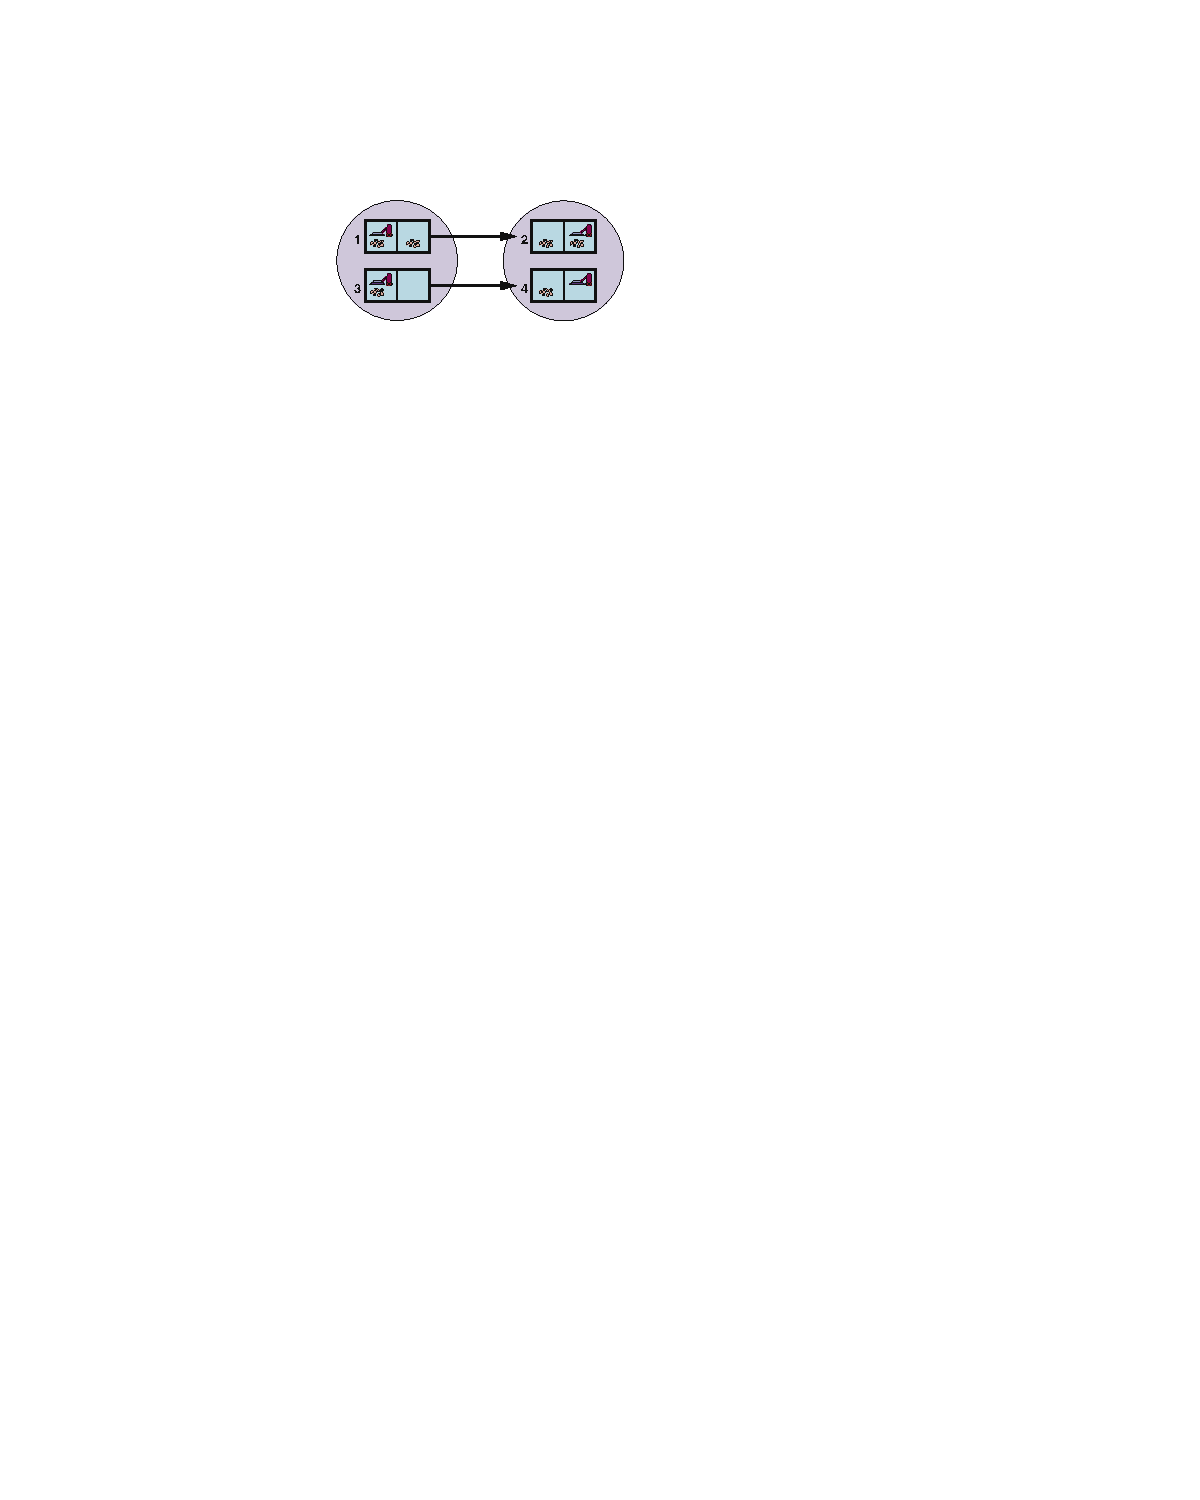
\includegraphics[alt={aima fig 04_13_a sensorless vacuum belief state deterministic actions},width=0.75\linewidth]{aima-fig-04_13_a-sensorless-vacuum-belief-state-deterministic-actions.pdf}



\begin{align*}
b' = Result(b,a)             &= \{s': s' = Result_P(s,a) \text{ and } s \in b\}\\
b' = Result(\{1, 3\}, Right) &= \{ Result_P(1,Right), Result_P(3,Right) \}\\
                             &= \{2, 4\}
\end{align*}
\section{Predicting Belief States in Sensorless Slippery Vacuum World}
\label{sec:org320666a}

Apply the nondeterministic action to all states in \(b\) to get \(b'\).


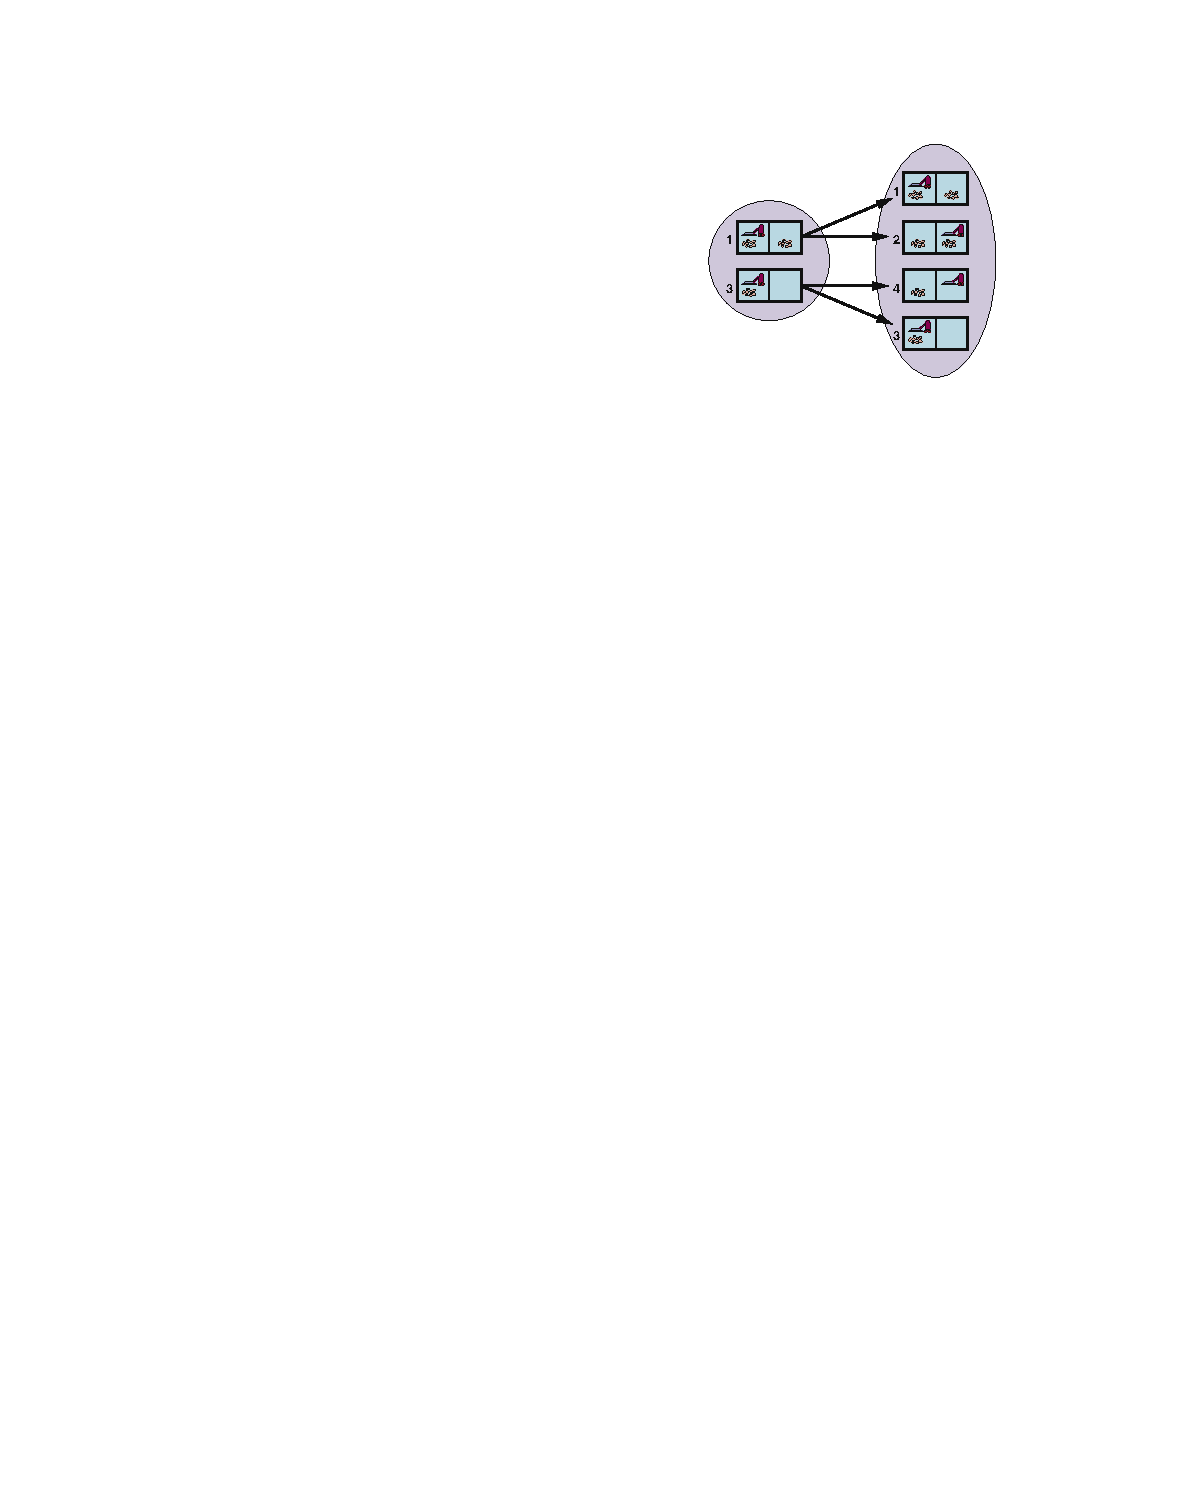
\includegraphics[alt={aima fig 04_13_b sensorless vacuum belief state nondeterministic actions},width=0.75\linewidth]{aima-fig-04_13_b-sensorless-vacuum-belief-state-nondeterministic-actions.pdf}


\begin{align*}
b'= Results(b,a)             &= \bigcup_{s \in b} Results_P(s,a)\\
b' = Result(\{1, 3\}, Right) &= \bigcup_{s \in \{1, 3\}} Results_P(s,Right)\\
b' = Result(\{1, 3\}, Right) &= Result_P(1,Right) \cup Result_P(3,Right)\\
                             &= \{1, 2\} \cup \{4, 3\}\\
                             &= \{1, 2, 4, 3\}
\end{align*}
\section{Search in Partially Observable Environments}
\label{sec:orgdc4ad13}

Many problems cannot be solved without sensing, e.g., sensorless 8-puzzle is impossible.

We can solve 8-puzzles if we can see just the upper-left corner square by moving each tile in turn into the observable square and keeping track of its location from then on.

For a partially observable problem, the problem specification will specify a \(Percept(s)\) function that returns the percept received by the agent in a given state.

\begin{itemize}
\item For nondeterministic sensing, \(Percepts(s) = \{s\}_{s \in S}\)
\item For fully observable problems, \(\forall s, Percept(s) = s\)
\item For sensorless problems \(Percept(s) = \text{null}\).
\end{itemize}
\section{Local-Sensing Vacuum World}
\label{sec:orga935d16}




The agent has a position sensor that yields the percept L in the left square, and R in the right square, and a dirt sensor that yields Dirty when the current square is dirty and Clean when it is clean -- but does not sense the other square.  This is nondeterministic sensing becuase the same percept can match more than one state:

\begin{itemize}
\item The PERCEPT in State 1 is [L,Dirty].
\item State 3 will also produce [L,Dirty].
\item Hence, the initial belief state will be \{1,3\}:

\begin{itemize}
\item \(Percepts(1) = \{1, 3\}\)
\end{itemize}
\end{itemize}

How do we algorithmically get that belief state \ldots{}





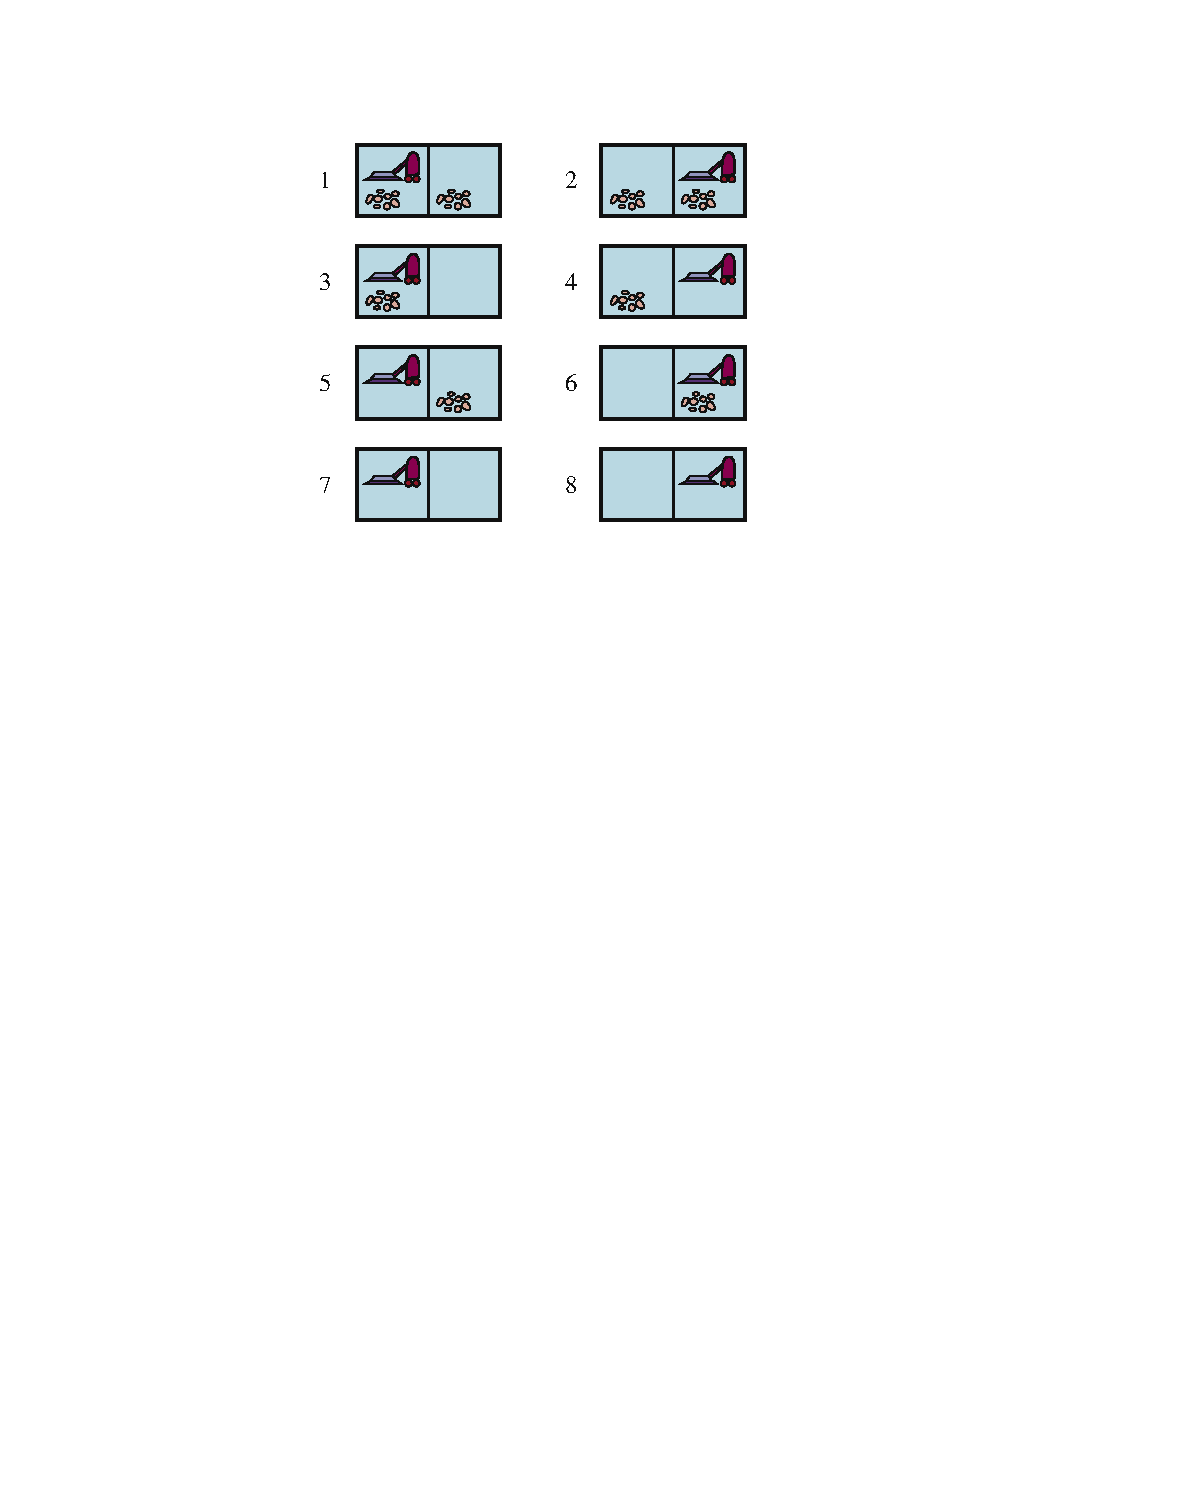
\includegraphics[alt={aima fig 04_09 vacuum states},width=0.75\linewidth]{aima-fig-04_09-vacuum-states.pdf}
\section{Transition Model in Partially Observable Environments}
\label{sec:org6c4f0d1}

After we apply an action in a given belief state, we can think of the transition model between belief states for partially observable problems as occurring in three stages, as depicted in the next slide:

\begin{itemize}
\item The \textbf{prediction} stage computes the belief state resulting from the action, Result(b,a), exactly as we did with sensorless problems. To emphasize that this is a prediction, we use the notation \(\hat{b} = Result(b,a)\), where the hat over the \(b\) means "estimated," and we also use Predict(b,a) as a synonym for Result(b,a).

\item The \textbf{possible percepts} stage computes the set of percepts that could be observed in the
\end{itemize}
predicted belief state (using the letter o for observation):

\begin{equation*}
PossiblePercepts(\hat{b}) = \{o : o = Percept(s) \text{ and } s \in \hat{b}\}
\end{equation*}

\begin{itemize}
\item The \textbf{update} stage computes, for each possible percept, the belief state that would result from the percept. The updated belief state \(b_o\) is the set of states in \(\hat{b}\) that could have
\end{itemize}
produced the percept:

\begin{equation*}
b_o = Update(\hat{b},o) = \{s : o = Percept(s) \text{ and } s \in \hat{b}\}
\end{equation*}
\section{State Transitions with Local Sensing (Summary)}
\label{sec:org426d5d5}




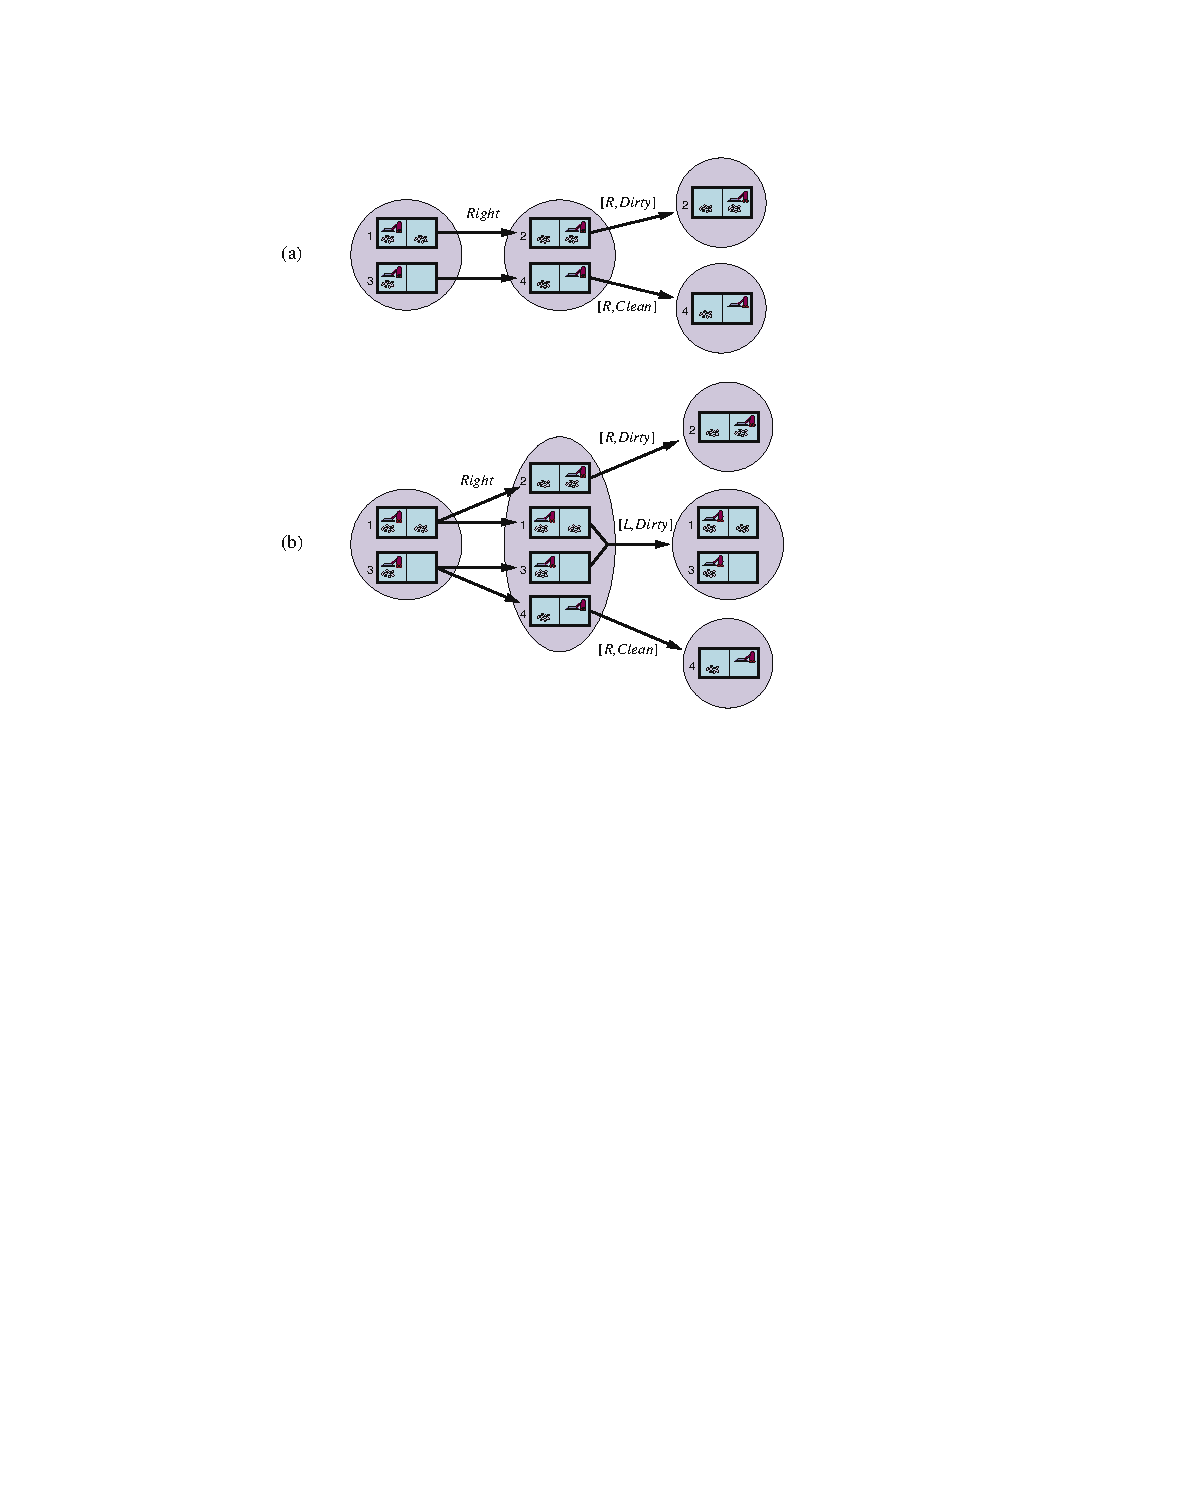
\includegraphics[alt={aima fig 04_15 local sensing vacuum state transitions},width=0.75\linewidth]{aima-fig-04_15-local-sensing-vacuum-state-transitions.pdf}





\begin{enumerate}
\item Predict \(\hat{b} = Result(b, a)\)
\end{enumerate}
\begin{multline*}
\text{2. } PossiblePercepts(\hat{b}) = \\
\{o : o = Percept(s) \text{ and } s \in \hat{b}\}
\end{multline*}
\begin{multline*}
\text{3. } b_o = Update(\hat{b},o) = \\
\{s : o = Percept(s) \text{ and } s \in \hat{b}\}
\end{multline*}


Final column on left shows input to Update step, which will then compute the final \(b_o\) based on percept/observation \(o\).

\begin{itemize}
\item (a) Deterministic world.
\item (b) Slippery world. Input to Update step are 3 belief states, each of which is no larger than the belief state from which they were produced.
\end{itemize}
\section{State Transitions with Local Sensing and Deterministic Actions}
\label{sec:org913e6c6}




\begin{enumerate}
\item Predict:
\end{enumerate}
\vspace{-.25in}
\begin{align*}
\hat{b} &= Result(b, a)\\
        &= Result(\{1, 3\}, Right)\\
        &= \{2, 4\}
\end{align*}

\begin{enumerate}
\item Possible percepts:
\end{enumerate}
\vspace{-.25in}
\begin{align*}
PossiblePercepts(\hat{b})  &= \{o : o = Percept(s) \text{ and } s \in \hat{b}\}\\
PossiblePercepts(\{2, 4\}) &= \{o : o = Percept(s) \text{ and } s \in \{2, 4\}\}\\
                           &= \{[R, Dirty], [R, Clean]\}
\end{align*}





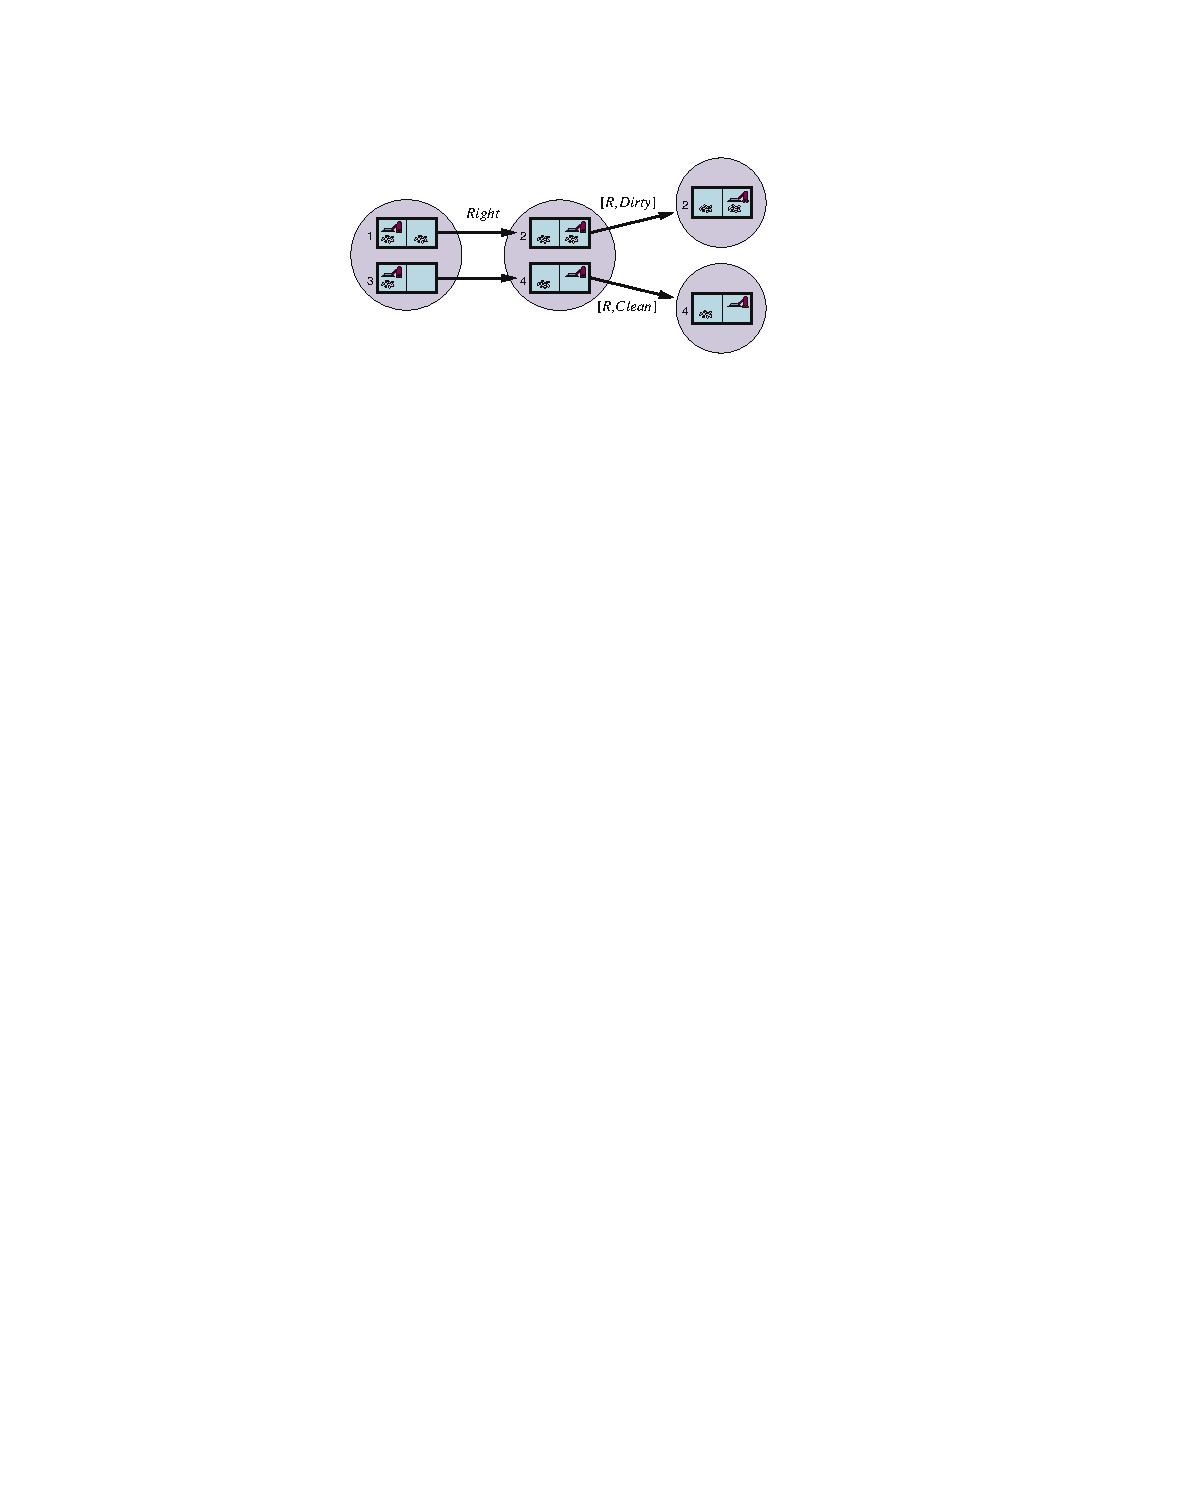
\includegraphics[alt={aima fig 04_15_a local sensing vacuum deterministic state transitions},width=0.75\linewidth]{aima-fig-04_15_a-local-sensing-vacuum-deterministic-state-transitions.pdf}





Then the two belief states on the right are then fed to the final step once the agent gets a percept.  If the percept is \([R, Dirty]\), then:

\begin{enumerate}
\item Update:
\end{enumerate}
\vspace{-.25in}
\begin{align*}
b_o &= Update(\hat{b},o) = \{s : o = Percept(s) \text{ and } s \in \hat{b}\}\\
    &= Update(\{[R, Dirty], [R, Clean]\}) = \{s : o = Percept(s) \text{ and } s \in \hat{b}\}\\
    &= \{2\}
\end{align*}
\section{State Transitions with Local Sensing in Slippery Vacuum World}
\label{sec:org248dd97}




\begin{enumerate}
\item Predict:
\end{enumerate}
\vspace{-.25in}
\begin{align*}
\hat{b} &= Result(b, a)\\
        &= Result(\{1, 3\}, Right)\\
        &= \{2, 1, 3, 4\}
\end{align*}

\begin{enumerate}
\item Possible percepts:
\end{enumerate}
\vspace{-.25in}
\[
PossiblePercepts(\hat{b}) = \{o : o = Percept(s) \text{ and } s \in \hat{b}\}
\]
\vspace{-.4in}
\begin{multline*}
PossiblePercepts(\{2, 1, 3, 4\}) = \\
    \{o : o = Percept(s) \text{ and } s \in \{2, 1, 3, 4\}\} =\\
    \{[R, Dirty], [L, Dirty], [L, Dirty], [R, Clean]\}
\end{multline*}






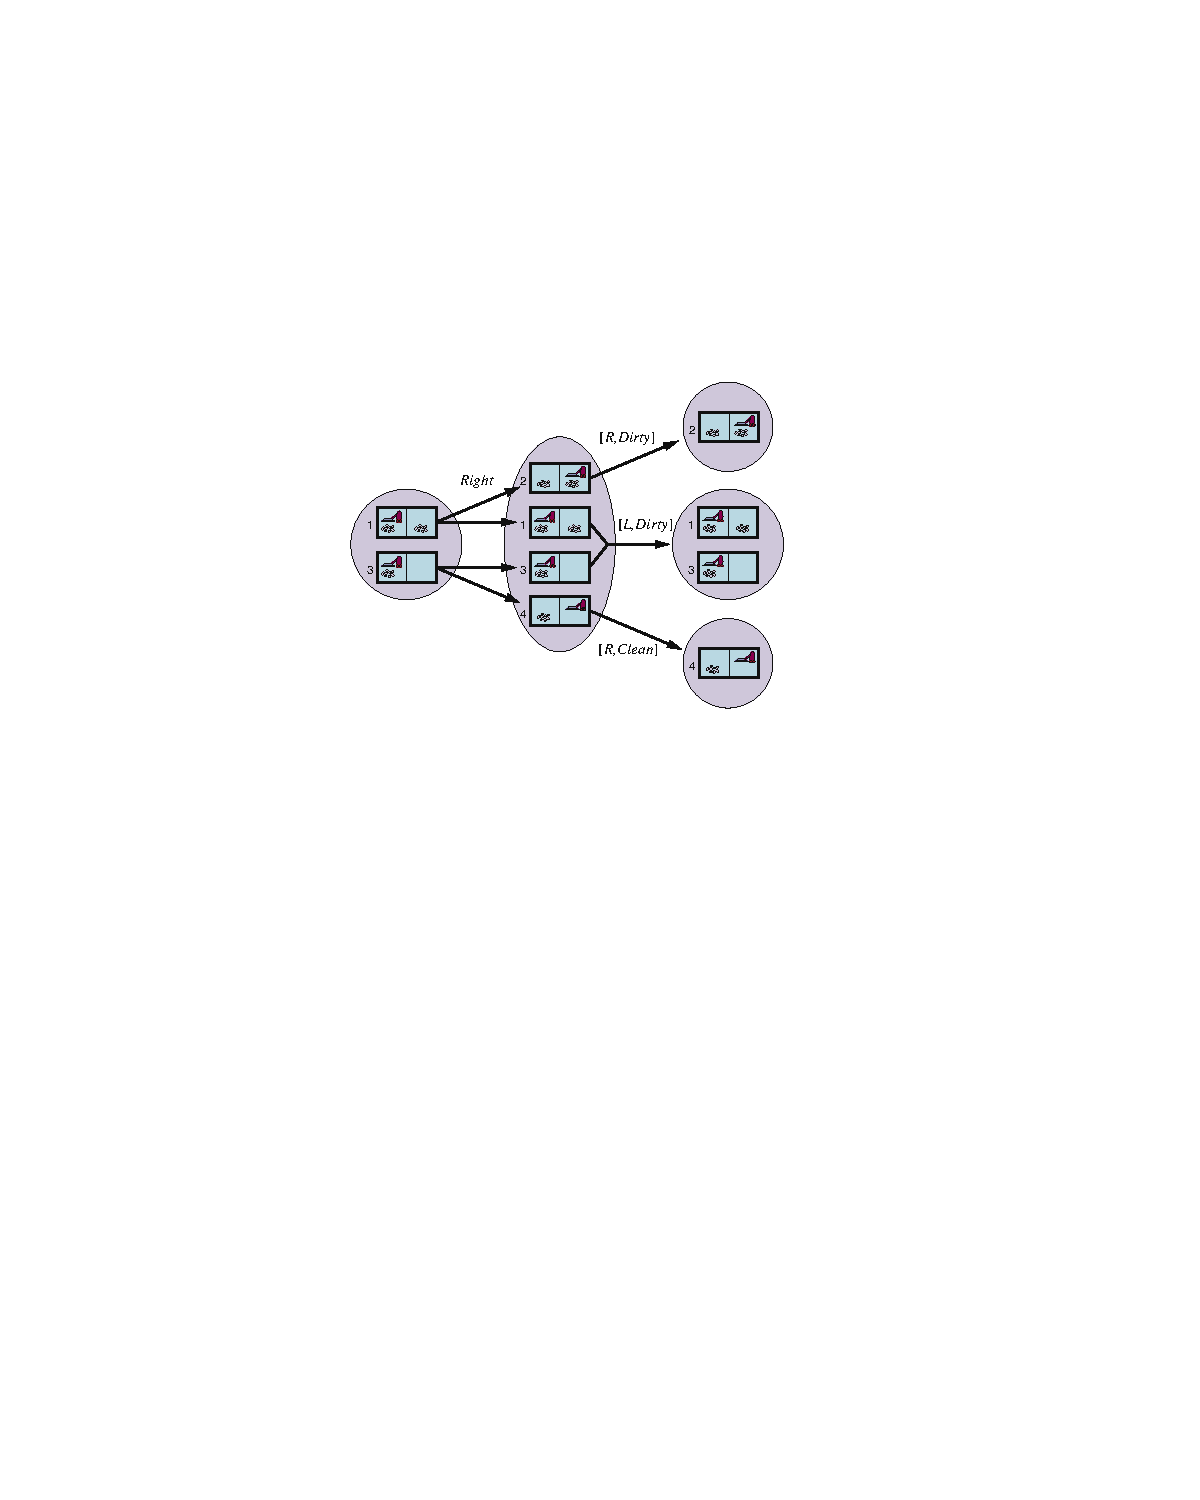
\includegraphics[alt={aima fig 04_15_b local sensing vacuum nondeterministic state transitions},height=2.0in]{aima-fig-04_15_b-local-sensing-vacuum-nondeterministic-state-transitions.pdf}





Then the three belief states on the right are then fed to the final step once the agent gets a percept.  If the percept is \([L, Dirty]\), then:

\begin{enumerate}
\item Update:
\end{enumerate}
\vspace{-.25in}
\begin{align*}
b_o &= Update(\hat{b},o) = \{s : o = Percept(s) \text{ and } s \in \hat{b}\}\\
    &= Update(\{[R, Dirty], [L, Dirty], [L, Dirty], [R, Clean]\}) = \{s : o = Percept(s) \text{ and } s \in \hat{b}\}\\
    &= \{1, 3\}
\end{align*}
\section{Planning Time State Estimation}
\label{sec:orgdcc937a}

The agent needs to deal with possible percepts at planning time, because it won’t know the actual percepts until it executes the plan.

\begin{itemize}
\item Nondeterminism in the physical environment can enlarge the belief state in the prediction stage, but each updated belief state \(b_o\) can be no larger than the predicted belief state \(\hat{b}\); observations can only help reduce uncertainty.
\item For deterministic sensing, the belief states for the different possible percepts will be disjoint, forming a partition of the original predicted belief state.
\end{itemize}

Putting the three stages from previous slide together, we obtain the possible belief states resulting from a given action and the subsequent possible percepts:

\begin{equation*}
Results(b,a) = \{b_o : b_o = Update(Predict(b,a),o) \text{ and }
    o \in PossiblePercepts(Predict(b,a))\}.
\end{equation*}
\section{Belief State Maintenance in Partially Observable Environments}
\label{sec:org09c8f8a}

Kindergarten world (square not being actively cleaned can become dirty):

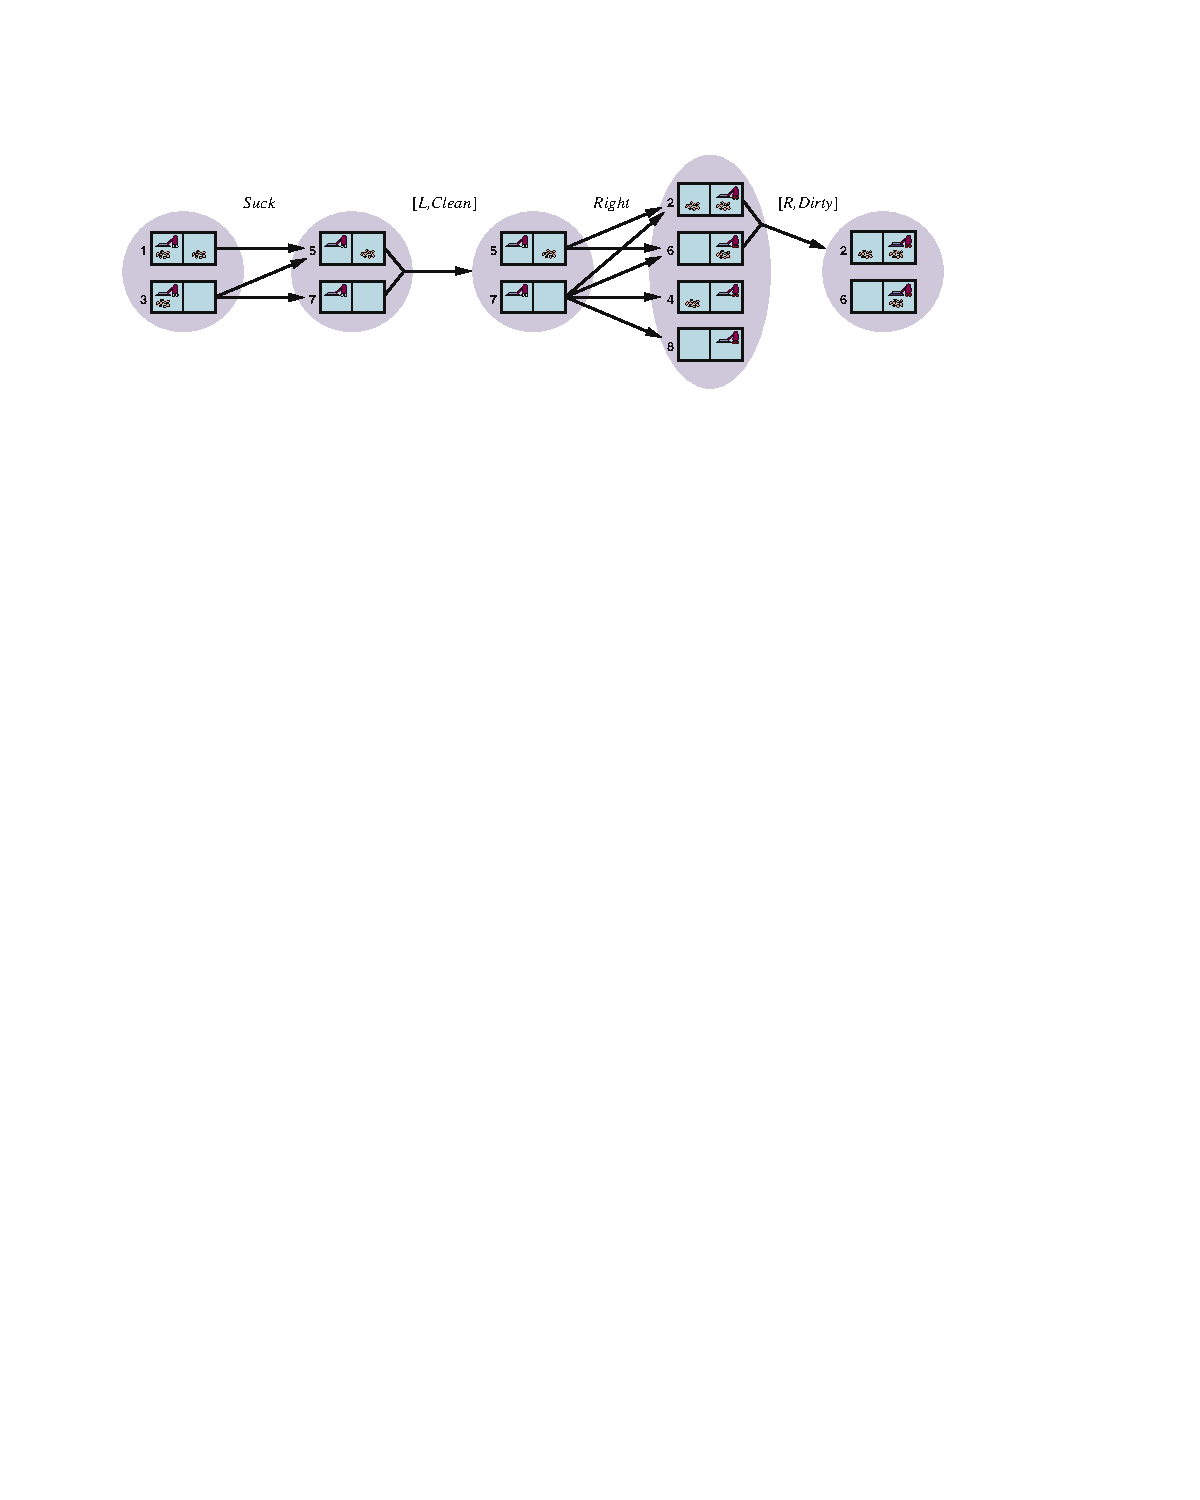
\includegraphics[alt={aima fig 04_17 vacuum prediction update cycles},width=0.75\linewidth]{aima-fig-04_17-vacuum-prediction-update-cycles.pdf}


\begin{itemize}
\item Most real-world environments partially observable.  Belief state maintenance is core task.
\item Also known as \textbf{monitoring}, \textbf{filtering}, and \textbf{state estimation}.
\end{itemize}

\begin{equation*}
b' = Update(Predict(b,a),o).
\end{equation*}

Equation above is called a recursive state estimator because it computes the new belief state from the previous one rather than by examining the entire percept sequence.
\section{Robot Localization}
\label{sec:org354b6d5}

Localization: typical robot state estimation problem in which the robot works out where it is, given a map of the world and a sequence of percepts and actions.


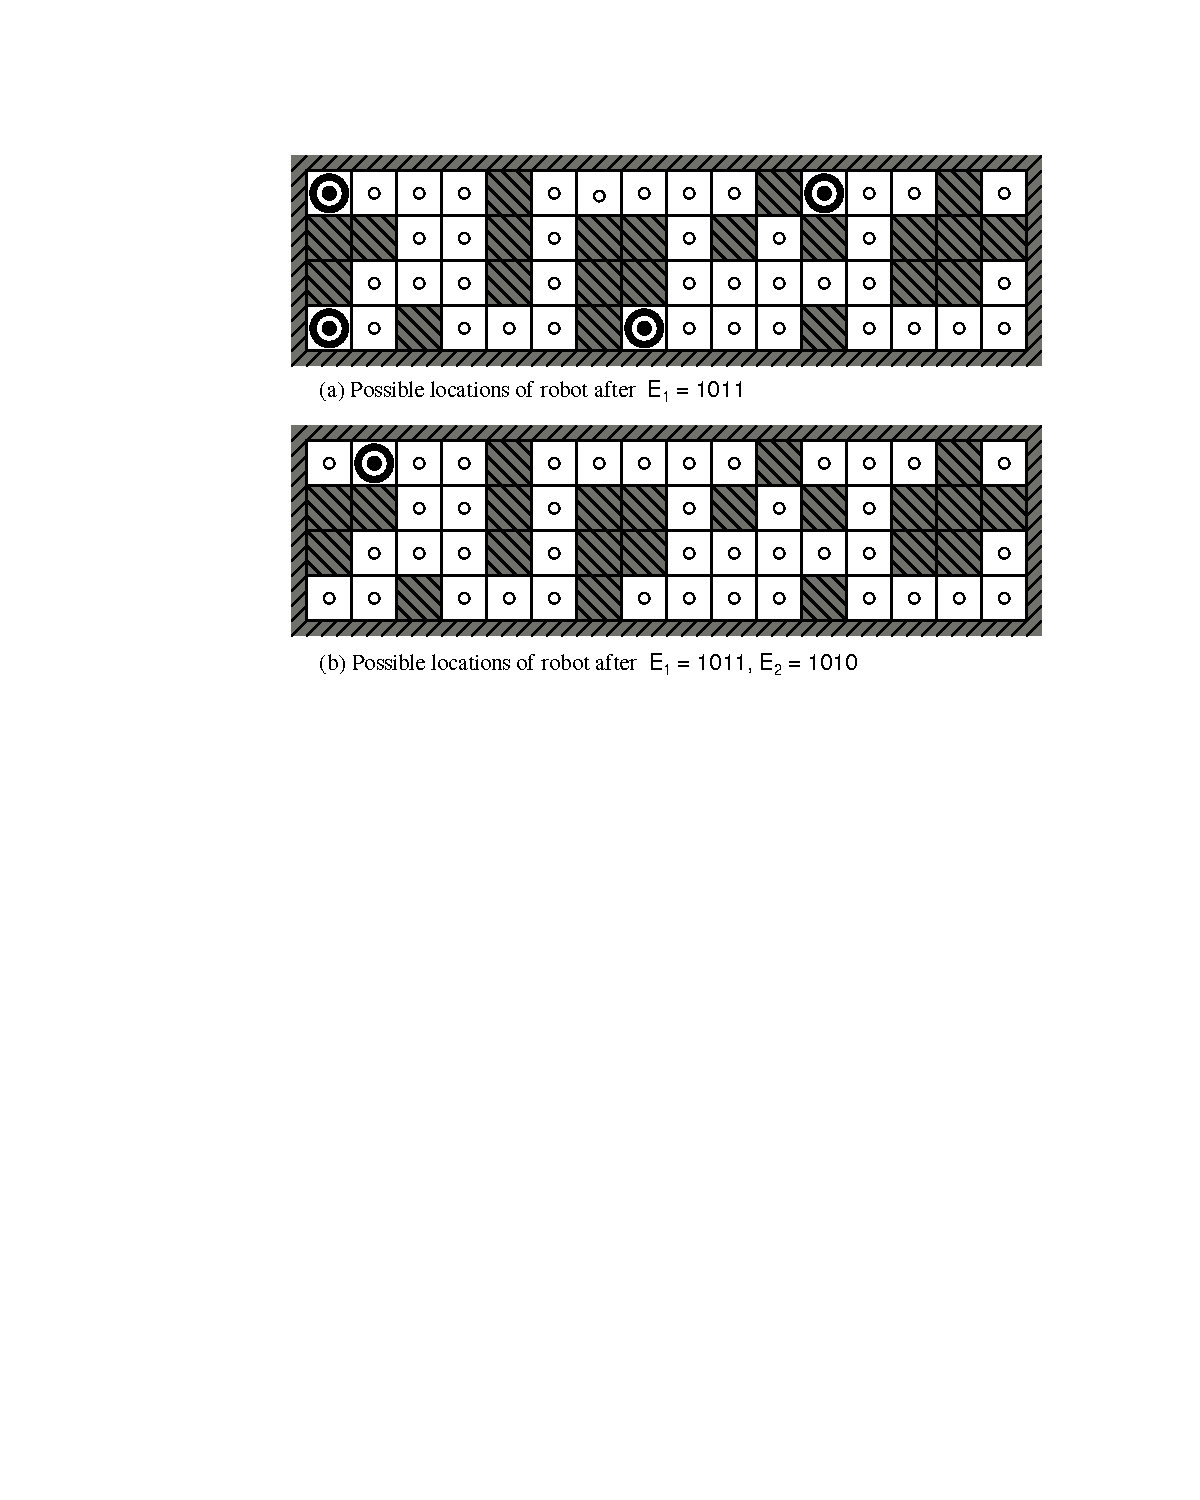
\includegraphics[alt={aima fig 04_18 robot localization},height=2.4in]{aima-fig-04_18-robot-localization.pdf}
\section{Online Seach}
\label{sec:org145623d}

\begin{itemize}
\item Agents we've studied so far use \textbf{offline search} algorithms, which compute a complete solution before taking first action.
\item \textbf{Online search} agents interleave computation and action.

\begin{itemize}
\item Good in dynamic environments where computation time must be limited so environment doesn't change while the agent computes an action.
\item Good in nondeterministic environments so agent can focus on contingencies that actually arise.
\item In unkown environments, agent must act in order to learn about the environment.
\item Tradeoff: more planning can prevent ending up in dead ends.
\end{itemize}
\end{itemize}

Canonical example of online search: mapping problem.  Agent placed in unknown environment and must explore to build a map.

\begin{itemize}
\item The problem of doing localization and mapping at the same time is called \textbf{SLAM}: Simultaneous Localization and Mapping.
\end{itemize}
\end{document}
